\documentclass[11pt]{article}           
\usepackage[UTF8]{ctex}
\usepackage[a4paper]{geometry}
\geometry{left=2.0cm,right=2.0cm,top=2.5cm,bottom=2.5cm}

\usepackage{xcolor}
\usepackage{paralist}
\usepackage{enumitem}
\setenumerate[1]{itemsep=0pt,partopsep=0pt,parsep=0pt,topsep=0pt}
\setitemize[1]{itemsep=0pt,partopsep=0pt,parsep=0pt,topsep=0pt}
\usepackage{comment}
\usepackage{booktabs}
\usepackage{graphicx}
\usepackage{float}
\usepackage{diagbox}
\usepackage{amsmath,amsfonts,graphicx,amssymb,bm,amsthm}
%\usepackage{algorithm,algorithmicx}
\usepackage[ruled]{algorithm2e}
\usepackage[noend]{algpseudocode}
\usepackage{fancyhdr}
\usepackage{tikz}
\usepackage{graphicx}
\usetikzlibrary{arrows,automata}
\usepackage[hidelinks]{hyperref}
\usepackage{extarrows}
\usepackage{lastpage}
\usepackage{totcount}
\setlength{\headheight}{14pt}
\setlength{\parindent}{0 in}
\setlength{\parskip}{0.5 em}
\usepackage{helvet}
\usepackage{dsfont}
\usepackage{threeparttable}
\usepackage{multirow}
\usepackage{tabularx}
\usepackage{makecell}
\usepackage{caption}
% \usepackage{newtxmath}

\newtheorem{theorem}{Theorem}
\newtheorem{lemma}[theorem]{Lemma}
\newtheorem{proposition}[theorem]{Proposition}
\newtheorem{claim}[theorem]{Claim}
\newtheorem{corollary}[theorem]{Corollary}
\newtheorem{definition}[theorem]{Definition}
\newtheorem*{definition*}{Definition}

\newenvironment{problem}[2][Problem]{\begin{trivlist}
\item[\hskip \labelsep {\bfseries #1}\hskip \labelsep {\bfseries #2.}]\songti}{\hfill$\blacktriangleleft$\end{trivlist}}
\newenvironment{answer}[1][Solution]{\begin{trivlist}
\item[\hskip \labelsep {\bfseries #1.}\hskip \labelsep]}{\hfill$\lhd$\end{trivlist}}

\newcommand\1{\mathds{1}}
% \newcommand\1{\mathbf{1}}
\newcommand\R{\mathbb{R}}
\newcommand\E{\mathbb{E}}
\newcommand\N{\mathbb{N}}
\newcommand\NN{\mathcal{N}}
\newcommand\per{\mathrm{per}}
\newcommand\PP{\mathbb{P}}
\newcommand\dd{\mathrm{d}}
\newcommand\Var{\mathrm{Var}}
\newcommand\Cov{\mathrm{Cov}}
\newcommand{\Exp}{\mathrm{Exp}}
\newcommand{\arrp}{\xrightarrow{P}}
\newcommand{\arrd}{\xrightarrow{d}}
\newcommand{\arras}{\xrightarrow{a.s.}}
\newcommand{\arri}{\xrightarrow{n\rightarrow\infty}}

\title{Homework \#3}
\usetikzlibrary{positioning}

\begin{document}
\kaishu

\pagestyle{fancy}
\lhead{\CJKfamily{zhkai} 北京大学}
\chead{}
\rhead{\CJKfamily{zhkai} 2024年秋\ 社会统计学(张春泥)}
\fancyfoot[C]{\thepage\ /\ \pageref{LastPage} \\ \textcolor{lightgray}{最后编译时间: \today}}



\begin{center}
    {\LARGE \bf Homework 3}

    {姓名:方嘉聪\ \  学号: 2200017849}            % Write down your name and ID here.
\end{center}
\begin{problem}{1}
    表 \ref{tab:1.1} 是2016年美国大选后CNN 网站发布的出口民调(exit polls)的数据统计. 出口民调是对一部分已投票选民所做的问卷调查, 调查内容包括选民的社会人口特征、政治态度和投票结果等信息, 出口民调的数据可以用来预测总体或某些群体的选民的投票结果, 也可以用于分析选民特征与投票的关系. 比如, 根据出口民调的数据, 我们可以推断2016年美国大选中什么特征的选民会支持希拉里·克林顿(Clinton), 什么特征的选民会支持唐纳德·特朗普(Trump). 
    \begin{table}[H]
        \centering
        \caption{选民受教育程度与投票对象 (\%) ($N=24558$)}
        \label{tab:1.1}
        \begin{tabularx}{0.8\textwidth}{l>{\centering\arraybackslash}X>{\centering\arraybackslash}X>{\centering\arraybackslash}X}
            \hline
            \textbf{} & \textbf{Clinton \%} & \textbf{Trump \%} & \textbf{其他/不回答 \%} \\
            \hline
            高中或以下 & \multirow{2}{*}{46} & \multirow{2}{*}{51} & \multirow{2}{*}{3} \\
            high school or less (18\%) & & & \\
            大学未毕业 & \multirow{2}{*}{43} & \multirow{2}{*}{52} & \multirow{2}{*}{6} \\
            some college (32\%) & & & \\
            大学毕业 & \multirow{2}{*}{49} & \multirow{2}{*}{44} & \multirow{2}{*}{7} \\
            college graduate (32\%) & & & \\
            研究生 & \multirow{2}{*}{58} & \multirow{2}{*}{37} & \multirow{2}{*}{5} \\
            postgraduate (18\%) & & & \\
            \hline
        \end{tabularx}
    \end{table} 
    根据表 \ref{tab:1.1}, 请回答以下问题:
    \begin{enumerate}[label=(\arabic*)]
        \item 简要陈述表 \ref{tab:1.1} 所描述的统计关系, 并指出这组关系中暗含的自变量是什么?
        \item 将表 \ref{tab:1.1} 还原为列联频次表, 要求这张表仅统计支持了Clinton或Trump的受访选民(即排除掉不回答或者支持 “其他”的受访者), 表中应展示行和列的合计频次.  {\kaishu (提示: 如遇人数非整数的情况, 请四舍五入保留整数)}
        \item 如果以受教育程度反映选民的社会经济地位, 基于(2)构造的列联表, 请检验美国选民在支持Clinton和Trump上是否存在精英选民和底层选民之间的差异?针对这一研究问题, 写出原假设和备择假设、期望频次分布、卡方值、自由度和统计显著性检验的结果(设显著性水平为0.01). 
    \end{enumerate}
\end{problem}
\begin{answer}
    \begin{enumerate}[label=(\arabic*)]
        \item 表 \ref{tab:1.1} 描述了2016年美国大选选民受教育程度与投票对象的关系. 暗含的自变量是选民受教育程度. \textcolor{red}{注意: 表格中已经给出数据, 我们需要明确地给出自变量和因变量之间具体存在什么关系, 正/负相关, 或什么倾向. }
        \item 列联频次表见表 \ref{tab:1.2} (表中数据保留整数).
        \item 为检验题述问题, 原假设与备择假设如下:
        \begin{align*}
            H_0&: \text{美国选民在支持Clinton和Trump上 \underline{不存在} 精英选民和底层选民之间的差异} \\
            H_1&: \text{美国选民在支持Clinton和Trump上 \underline{存在} 精英选民和底层选民之间的差异}
        \end{align*}
        期望联合频次分布表见表 \ref{tab:1.3}. 
        \begin{table}[H]
            \centering
            \caption{选民受教育程度与投票对象的列联频次表(人), 美国总统大选, 2016}
            \label{tab:1.2}
            \begin{tabularx}{0.8\textwidth}{l>{\centering\arraybackslash}X>{\centering\arraybackslash}X>{\centering\arraybackslash}X}
                \hline
                \textbf{} & \textbf{Clinton } & \textbf{Trump} & \textbf{合计} \\
                \hline
                高中或以下 & \multirow{2}{*}{2033} & \multirow{2}{*}{2254} & \multirow{2}{*}{4287} \\
                high school or less  & & & \\
                大学未毕业 & \multirow{2}{*}{3379} & \multirow{2}{*}{4086} & \multirow{2}{*}{7465} \\
                some college  & & & \\
                大学毕业 & \multirow{2}{*}{3851} & \multirow{2}{*}{3458} & \multirow{2}{*}{7309} \\
                college graduate  & & & \\
                研究生 & \multirow{2}{*}{2564} & \multirow{2}{*}{1636} & \multirow{2}{*}{4200} \\
                postgraduate  & & & \\
                合计 & 11827 & 11434 & 23261 \\
                \hline
            \end{tabularx}
        \end{table}
        \begin{table}[H]
            \centering
            \caption{选民受教育程度与投票对象的期望频次分布表(人), 美国总统大选, 2016}
            \label{tab:1.3}
            \begin{tabularx}{0.8\textwidth}{l>{\centering\arraybackslash}X>{\centering\arraybackslash}X>{\centering\arraybackslash}X}
                \hline
                \textbf{} & \textbf{Clinton } & \textbf{Trump} & \textbf{合计} \\
                \hline
                高中或以下 & \multirow{2}{*}{2180} & \multirow{2}{*}{2107} & \multirow{2}{*}{4287} \\
                high school or less  & & & \\
                大学未毕业 & \multirow{2}{*}{3796} & \multirow{2}{*}{3670} & \multirow{2}{*}{7465} \\
                some college  & & & \\
                大学毕业 & \multirow{2}{*}{3716} & \multirow{2}{*}{3593} & \multirow{2}{*}{7309} \\
                college graduate  & & & \\
                研究生 & \multirow{2}{*}{2135} & \multirow{2}{*}{2065} & \multirow{2}{*}{4200} \\
                postgraduate  & & & \\
                合计 & 11827 & 11434 & 23261 \\
                \hline
            \end{tabularx}
        \end{table}
        那么
        \begin{align*}
            \chi^2&= \sum_i\sum_j \frac{(F_{ij}-E_{ij})^2}{E_{ij}} \approx 298.17\\ 
            df=(r-1)&(c-1)=3, \implies \chi^2_{0.01}(3) = 11.345 < \chi^2 
        \end{align*}
        故拒绝原假设, 即在显著性水平0.01下, 美国选民在支持Clinton和Trump上存在精英选民和底层选民之间的显著差异.
    \end{enumerate}
\end{answer}

\begin{problem}{2}
    工作-家庭冲突(work-family conflict)是指工作与家庭生活之间不协调造成的角色冲突和压力, 包括工作对家庭的干扰(work Interfering family, WIF)和家庭对工作的干扰(family Interfering work, FIW). 个体承受的WIF或FIW水平均可通过量表测量. 过往研究发现, 女性比男性承受了更高的工作-家庭冲突水平. 以往研究还发现, 工作-家庭冲突水平不仅与个体或家庭特征有关, 还可能与社会环境中的性别不平等程度有关. 在国家/地区层次, 衡量一国/地区性别不平等状况通常使用联合国开发计划署(UNDP)的性别不平等指数(Gender Inequality Index, 简称GII)这一综合性指标, 该指标取值从0到1, 得分越高表示该国家/地区性别不平等程度越高(即女性相对于男性处于不利地位). 
    
    现有一项研究试图探讨和检验国家/地区层次的性别平等环境与女性承受的工作-家庭冲突水平之间的关系. 表2(见excel数据)是参加2012年国际社会调查项目(ISSP)的39个国家的GII得分(设为$X$)和根据各国ISSP调查数据分别汇总的女性平均WIF评分的标准化得分(设为 $Y$). 

    根据表2数据, 请回答:
    \begin{enumerate}[label=(\arabic*)]
        \item 分布别计算 $\sum X, \sum Y, \sum XY, \sum X^2, \sum Y^2$.
        \item 根据 (1) 分别计算 $X,Y$ 的均值和方差, 以及两者的协方差 $\Cov(X,Y)$.
        \item 计算及解读两者的相关系数和判定系数, 并检验总体中国家/地区性别不平等指数与女性工作-冲突平均水平之间是否存在正相关(设显著性水平为0.05). 
        \item 根据题意, 以GII得分和女性WIF得分两个变量建立一元线性回归方程, 估计该方程的回归系数, 以公式形式表达. 
        \item 将GII得分按照$[0,0.1)、[0.1,0.2)、[0.2,1]$分成三组, 分别表示国家/地区性别不平等程度的低、中、高三个水平, 计算各水平组别的样本数、女性WIF得分的均值和方差, 以表格形式报告. 
        \item 根据(5), 用方差分析检验性别不平等水平为低、中、高三个组别的国家/地区是否在女性工作-家庭冲突水平上存在显著差异(设显著性水平为0.05). 
        \item 图1是39个国家GII指数(横轴)和女性WIF平均得分(纵轴)的散点图, 根据上述一系列分析及结合该散点图, 简要总结研究发现, 并尝试评论为何这两个变量之间的判定系数较小{\kaishu(提示: 言多必失, 意思表达清楚即可)}
        \begin{figure}[H]
            \centering
            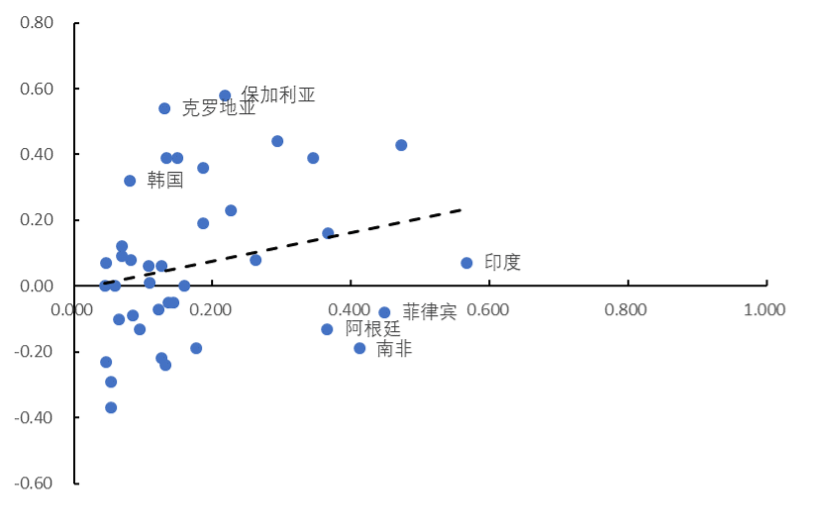
\includegraphics[width=0.6\textwidth]{Picture1.png}
            \caption*{\footnotesize 注: 每个散点代表一个国家, 有少数国家标记了国家名称, 其余未标记. 虚线为估计的回归直线}
            \caption{各国GII和女性平均WIF得分的散点图及回归直线}
            \label{fig:1.1}
        \end{figure}
    \end{enumerate}
\end{problem}
\begin{answer} 
    \begin{enumerate}[label=(\arabic*)]
        \item 计算结果如下:
        \begin{align*}
            \sum X = 6.96, \quad \sum Y = 2.63, \quad \sum XY =  0.76, \quad \sum X^2 =  1.93, \quad \sum Y^2 =  2.38.
        \end{align*}
        \item 以下计算均为为样本数值, $n = 39$:
        \begin{align*}
            \bar{X} = \frac{\sum X}{n} = 0.18, \quad S_X^2 &= \frac{1}{n-1}\left(\sum X^2 - n \bar{X}^2\right) = 0.02, \\
            \bar{Y} = \frac{\sum Y}{n} = 0.07, \quad S_Y^2 &= \frac{1}{n-1}\left(\sum Y^2 - n \bar{Y}^2\right) = 0.06, \\
            \Cov(X,Y) = \frac{1}{n-1}&\sum (X_i-\bar{X})(Y_i-\bar{Y}) = 0.01.
        \end{align*}
        \item 相关系数和判定系数计算如下:
        \begin{align*}
            r = \frac{\Cov(X,Y)}{\sqrt{S_X^2S_Y^2}} = 0.24, \quad r^2 = 0.06.
        \end{align*}
        \textcolor{red}{(注意: 要具体给出解释, 认真审题!)}
        说明国家/地区性别不平等指数与女性工作-冲突平均水平两个变量之间可以相互解释 $6\%$ 的方差. 在总体中是否存在正相关, 需进一步检验, 原假设与备择假设如下:
        \begin{align*}
            H_0&: \text{总体中国家/地区性别不平等指数与女性工作-冲突平均水平之间 \underline{不存在} 正相关\textcolor{red}{(这里应该是相关)}} \\
            H_1&: \text{总体中国家/地区性别不平等指数与女性工作-冲突平均水平之间 \underline{存在} 正相关}
        \end{align*}
        计算 $t$ 统计量如下:
        \begin{align*}
            t = r\sqrt{\frac{n-2}{1-r^2}} = 1.50, \quad \text{df} = n-2 = 37 \implies t_{0.05}(37) = 1.687 > t.
        \end{align*}
        故在显著性水平0.05下, 不能拒绝原假设, 即在显著性水平0.05下, 总体中国家/地区性别不平等指数与女性工作-冲突平均水平之间不存在正相关.
        \item 计算结果如下
        \begin{align*}
            b_1 = \frac{\Cov(X,Y)}{S_X^2} = 0.43, \quad b_0 = \bar{Y} - b_1\bar{X} = -0.01, \quad \hat{Y} = b_0 + b_1 X = -0.01 + 0.43X.
        \end{align*}
        \item 见表 \ref{tab:1.4}.
        \begin{table}[H]
            \centering
            \caption{国家/地区性别不平等程度的低、中、高水平样本分布及女性WIF得分的均值和方差}
            \label{tab:1.4}
            \begin{tabularx}{0.8\textwidth}{l>{\centering\arraybackslash}X>{\centering\arraybackslash}X>{\centering\arraybackslash}X}
                \hline
                \textbf{国家/地区性别不平等程度} & \textbf{样本数(个)} & \textbf{WIF 均值} & \textbf{WIF 方差} \\
                \hline
                低水平, $\text{GII} \in [0,0.1)$ & 13 & -0.04 & 0.04 \\
                中水平, $\text{GII} \in [0.1,0.2)$ & 15 & 0.08 & 0.06\\
                高水平, $\text{GII} \in [0.2,1]$ & 11 & 0.18 & 0.07 \\ 
                \hline
            \end{tabularx}
        \end{table}
        \item 原假设与备择假设如下:
        \begin{align*}
            H_0&: \text{性别不平等水平这三个组别的国家/地区在女性工作-家庭冲突水平上 \underline{不存在} 显著差异} \\
            H_1&: \text{性别不平等水平这三个组别的国家/地区在女性工作-家庭冲突水平上 \underline{存在} 显著差异}
        \end{align*}
        我们先来计算 BSS 和 WSS:
        \begin{align*}
            \text{TSS} = 2.20, \quad \text{BSS} = \sum_{g=1}^{3} n_g (\bar{y}_g - \bar{Y})^2  = 0.29, \quad \text{WSS} = \sum_{g=1}^{3} (n_g-1) s_g^2 = 1.91.
        \end{align*}
        进而计算 $F$ 统计量:
        \begin{align*}
            F = \frac{\text{BSS}/(G-1)}{\text{WSS}/(n-G)} = 2.76 < F_{0.05}(2,36) = 3.259.
        \end{align*}
        故在显著性水平0.05下, 不能拒绝原假设, 即在显著性水平0.05下, 性别不平等水平为低、中、高三个组别的国家/地区是否在女性工作-家
        庭冲突水平上不存在显著差异.
        \item \underline{总结:} 从上述计算可知, 在抽取的39个国家样本中, 国家/地区层次的性别平等环境与女性承受的工作-家庭冲突水平之间的存在较弱线性正相关关系. 但通过假设检验与方差分析的结果, 二者的这种线性正相关性在总体中并不显著.
        
        \underline{判定系数较小的原因猜测:} 观察散点图, 发现大部分数据点均偏离回归直线, 说明我们得到的这一回归方程并不能很好地解释数据的变异(欠拟合), 在总体上的线性正相关性不显著, 对应的判定系数较小. 

        女性工作-家庭冲突水平可能受到多种因素的影响, 例如女性收入, 家庭角色等, 不完全受到国家/地区性别不平等指数的影响. 此外散点图说明相关关系可能是 \underline{非线性的} , 也可能是多元的, 仅通过一个变量的线性回归模型难以很好地解释数据的变异.   
    \end{enumerate}
\end{answer}
\end{document}